\documentclass[a4paper]{article}

\usepackage{/c/tduong/home/tex/harvard/harvard}
%\VignetteIndexEntry{feature} 
\title{feature: R package}
\author{Tarn Duong}

\usepackage{/usr/lib/R/share/texmf/Sweave}
\begin{document}

\maketitle

\section{Introduction}

Feature significance is an extension of kernel density estimation, 
which is used to establish the statistical significance of 
features (like local modes). See \citeasnoun{chaudhuri99} for 1-dimensional data,
\citeasnoun{godtliebsen02} for  2-dimensional data and \citeasnoun{duong06}
for 3- and 4-dimensional data. \texttt{feature} is an R package for 
feature significance for 1- to 4-dimensional data.
  
There is one main function in this package, \texttt{featureSignif}. 
It has a range of options which allow
the user to compute and display kernel density estimates, significant gradient
and significant curvature regions. Significant gradient and/or
curvature regions often correspond to significant features. 
We cover the options which a newcomer would most likely require. 
For the full range of options (e.g. varying
plotting colours), see \texttt{?featureSignif}.


\section{Examples}
The earthquake data set is contained in 
\texttt{feature}. It contains 510 observations, each consisting
of measurements of an earthquake beneath the Mt St Helens volcano.
The first is the longitude (in degrees, where a negative number
indicates west of the International Date Line), second  is
the latitude (in degrees, where a positive number indicates north of
the Equator) and the third  is the depth (in km, where a
negative number indicates below the Earth's surface).

For the univariate example, we take the log --depth
as our variable of interest. 
Figure \ref{fig:fs1} contains the kernel
density estimate with bandwidth 0.1 (in orange). Superimposed in green 
are the sections of this density estimate which as significant gradient
(i.e. significantly different from zero). The rug plot is 
the log --depth measurements.

\begin{figure}
\begin{center}
\begin{Schunk}
\begin{Sinput}
> library(feature)
\end{Sinput}
\begin{Soutput}
Loading required package: KernSmooth
KernSmooth 2.22 installed
Copyright M. P. Wand 1997
Loading required package: misc3d
Loading required package: rgl
feature 1.1-3 1.0-0 (2006)
\end{Soutput}
\begin{Sinput}
> data(earthquake)
> eq3 <- -log10(-earthquake[, 3])
> featureSignif(eq3, addData = TRUE, addSignifGradRegion = TRUE, 
+     xlab = "-log(-depth)", bw = 0.1)
\end{Sinput}
\end{Schunk}
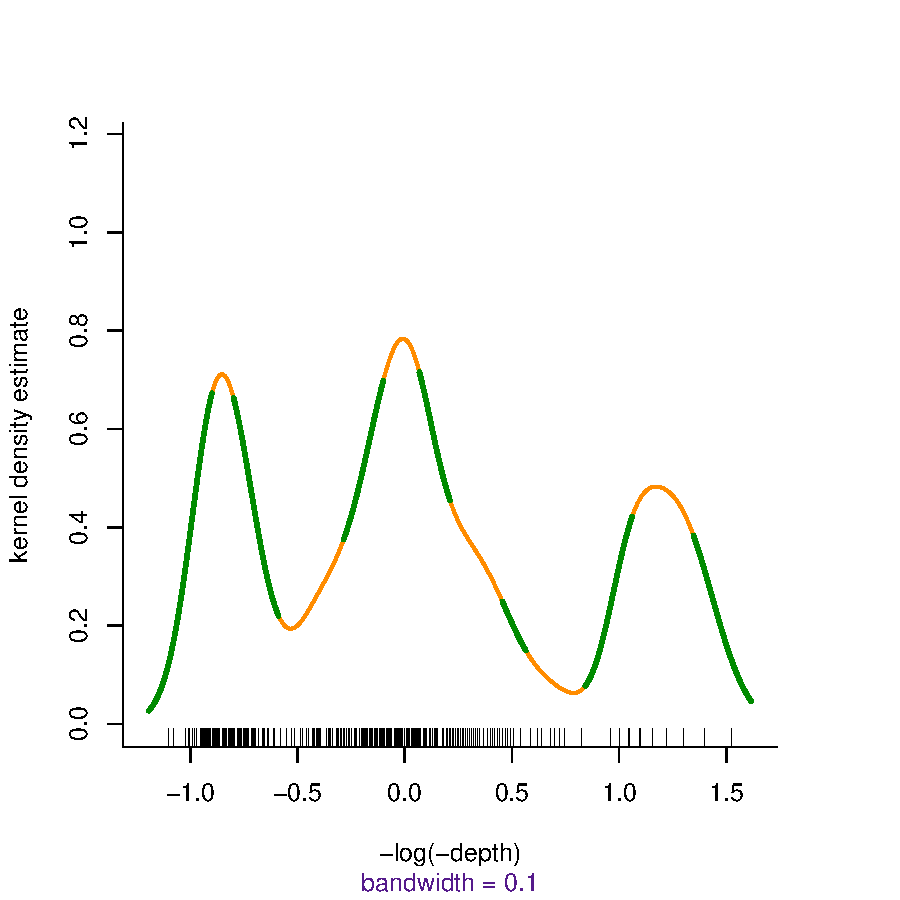
\includegraphics{feature-001}
\caption{Univariate data: significant gradient region with 
kernel density estimate}
\label{fig:fs1}
\end{center}
\end{figure}

Figure \ref{fig:fs2} contains the same kernel density estimate and 
significant gradient region plot along with the SiZer plot (cf. \citeasnoun{chaudhuri99}).
In the SiZer plot, blue indicates significantly increasing gradient,
red is significantly decreasing gradient, purple is non-significant gradient
and grey is data too sparse for reliable estimation. The horizontal black line
is for the bandwidth $0.1$.

\begin{figure}[!ht]
\begin{center}
\begin{Schunk}
\begin{Sinput}
> layout(matrix(1:2, nrow = 2))
> featureSignif(eq3, addSignifGradRegion = TRUE, xlab = "-log(-depth)", 
+     bw = 0.1)
> xlim <- par()$usr[1:2]
> featureSignif(eq3, plotSiZer = TRUE, xlab = "-log(-depth)", xlim = xlim)
> lines(c(-2, 2), c(0.1, 0.1))
> layout(1)
\end{Sinput}
\end{Schunk}
\includegraphics{feature-002}
\caption{Univariate data: significant gradient regions and SiZer plot}
\label{fig:fs2}
\end{center}
\end{figure}

\clearpage 
For bivariate data, we look at an Old Faithful geyser data set,
in the MASS library. The
horizontal axis is the waiting time (in minutes) between two eruptions, and
the vertical axis is the duration time (in minutes) of an eruption.
%The plot of the data with the kernel density estimate 
%with bandwidths (4.5, 0.37) is in Figure \ref{fig:fs3}
%\begin{figure}[!ht]
%\begin{center}
%library(MASS)
%data(geyser)
%featureSignif(geyser, addData=TRUE, bw=c(4.5, 0.37))
%\caption{Bivariate data: kernel density estimate}
%\label{fig:fs3}
%\end{center}
%\end{figure}
Figure \ref{fig:fs4} has a kernel density estimate with
bandwidth (4.5, 0.37), 
with the significant gradient regions in green
and the 
significant curvature regions in blue superimposed.
\begin{figure}[!ht]
\begin{center}
\begin{Schunk}
\begin{Sinput}
> library(MASS)
> data(geyser)
> featureSignif(geyser, addSignifGradRegion = TRUE, addSignifCurvRegion = TRUE, 
+     bw = c(4.5, 0.37))
\end{Sinput}
\end{Schunk}
\includegraphics{feature-003}
\caption{Bivariate data: significant gradient and curvature regions}
\label{fig:fs4}
\end{center}
\end{figure}

A variation on plotting the significant regions is to plot the data points which
fall inside these regions in Figure \ref{fig:fs5}: 
significant gradient data points are in green,  
significant curvature data points are in blue.
\begin{figure}[!ht]
\begin{center}
\begin{Schunk}
\begin{Sinput}
> fs <- featureSignif(geyser, addSignifGradData = TRUE, addSignifCurvData = TRUE, 
+     bw = c(4.5, 0.37))
\end{Sinput}
\end{Schunk}
\includegraphics{feature-004}
\caption{Bivariate data: significant gradient and curvature data points}
\label{fig:fs5}
\end{center}
\end{figure}

\clearpage
Usually \texttt{featureSignif} 
returns invisbly to R but in this example, we assigned it to the variable 
\texttt{fs}.
\begin{Schunk}
\begin{Sinput}
> names(fs)
\end{Sinput}
\begin{Soutput}
[1] "x"    "bw"   "fhat" "grad" "curv"
\end{Soutput}
\end{Schunk}
where x is the data, bw is the bandwidth, fhat\$est is the kernel density estimate
on the grid fhat\$x.grid, 
grad is the matrix indicating signficant gradient and 
curv is the matrix indicating signficant curvature. 
\begin{Schunk}
\begin{Sinput}
> fs$x[1:5, ]
\end{Sinput}
\begin{Soutput}
  waiting duration
1      80 4.016667
2      71 2.150000
3      57 4.000000
4      80 4.000000
5      75 4.000000
\end{Soutput}
\begin{Sinput}
> fs$bw
\end{Sinput}
\begin{Soutput}
[1] 4.50 0.37
\end{Soutput}
\begin{Sinput}
> fs$fhat$x.grid[[1]][30:35]
\end{Sinput}
\begin{Soutput}
[1] 51.42667 51.95000 52.47333 52.99667 53.52000 54.04333
\end{Soutput}
\begin{Sinput}
> fs$fhat$x.grid[[2]][101:106]
\end{Sinput}
\begin{Soutput}
[1] 4.096111 4.134289 4.172467 4.210644 4.248822 4.287000
\end{Soutput}
\begin{Sinput}
> fs$fhat$est[30:35, 101:106]
\end{Sinput}
\begin{Soutput}
           [,1]       [,2]       [,3]       [,4]       [,5]       [,6]
[1,] 0.01140390 0.01185379 0.01225223 0.01259516 0.01287930 0.01310208
[2,] 0.01169080 0.01214089 0.01253763 0.01287711 0.01315621 0.01337253
[3,] 0.01191348 0.01236082 0.01275322 0.01308690 0.01335892 0.01356710
[4,] 0.01207150 0.01251349 0.01289923 0.01322512 0.01348841 0.01368714
[5,] 0.01216557 0.01259999 0.01297718 0.01329373 0.01354706 0.01373545
[6,] 0.01219754 0.01262263 0.01298985 0.01329595 0.01353859 0.01371622
\end{Soutput}
\begin{Sinput}
> fs$grad[30:35, 101:106]
\end{Sinput}
\begin{Soutput}
     [,1] [,2] [,3]  [,4]  [,5]  [,6]
[1,] TRUE TRUE TRUE  TRUE  TRUE  TRUE
[2,] TRUE TRUE TRUE  TRUE  TRUE FALSE
[3,] TRUE TRUE TRUE  TRUE FALSE FALSE
[4,] TRUE TRUE TRUE  TRUE FALSE FALSE
[5,] TRUE TRUE TRUE FALSE FALSE FALSE
[6,] TRUE TRUE TRUE FALSE FALSE FALSE
\end{Soutput}
\begin{Sinput}
> fs$curv[30:35, 101:106]
\end{Sinput}
\begin{Soutput}
      [,1]  [,2]  [,3] [,4] [,5] [,6]
[1,] FALSE FALSE FALSE TRUE TRUE TRUE
[2,] FALSE FALSE FALSE TRUE TRUE TRUE
[3,] FALSE FALSE FALSE TRUE TRUE TRUE
[4,] FALSE FALSE  TRUE TRUE TRUE TRUE
[5,] FALSE FALSE FALSE TRUE TRUE TRUE
[6,] FALSE FALSE FALSE TRUE TRUE TRUE
\end{Soutput}
\end{Schunk}

\texttt{feature} includes 
feature significance for 3- and 4-dimensional
data. However the displays in these dimensions rely on the rgl \cite{rgl}
engine which is not quite integrated with \texttt{Sweave} 
so we have excluded examples for the time being. See 
the example code in \texttt{?featureSignif}.   
%so the 
%graphics are yet incorporated in this vignette.
%featureSignif(earthquake, scaleData=TRUE, addData=TRUE,
%    bw=c(0.0381, 0.0381, 0.0442))
%
%featureSignif(earthquake, addKDE=FALSE, scaleData=TRUE,
%   addSignifGradRegion=TRUE, addSignifCurvRegion=TRUE,
%   bw=c(0.0381, 0.0381, 0.0442),
%   xlim=c(0.4,0.5), ylim=c(0.4,0.5), zlim=c(0.8,0.9))

%data(iris) 
%featureSignif(iris[,1:4], addSignifGradData=TRUE,
%   addSignifCurvRegion=TRUE, bw=c(0.457, 0.210, 0.960, 0.413))

These examples have used \texttt{feature} in its non-interactive
mode where the user supplies a particular value of the bandwidth. 
In its interactive mode, the user is able to choose a
bandwidth from a range of bandwidths and the significant features are
displayed in real-time.
Again it's not possible to illustrate this nside this vignette,
see \texttt{?featureSignif}.   

%library(MASS)
%data(geyser)
%duration <- geyser$duration 
%featureSignif(duration, addSignifGradRegion=TRUE,
%   addSignifGradData=TRUE)
 

\bibliographystyle{agsm}
\bibliography{/c/tduong/home/research/references}
 

\end{document}
